
%\documentclass[letterpaper, 10 pt, conference]{ieeeconf}  % Comment this line out
                                                          % if you need a4paper
\documentclass[a4paper, 10pt, conference]{ieeeconf}      % Use this line for a4
\usepackage[pdftex]{graphicx}
\usepackage{nameref}

%%% LITTERATURLISTE %%%
\usepackage[square,numbers]{natbib}
\usepackage{url}

%For ÆØÅ
\usepackage[utf8]{inputenc}
\usepackage{nameref}

%For inserting a PDF into the report
\usepackage{pdfpages}

%equations
\usepackage{amsmath}

%\begin{comment}
\usepackage{verbatim}                
                
                                                          % paper

% \IEEEoverridecommandlockouts                              % This command is only
                                                          % needed if you want to
                                                          % use the \thanks command
% \overrideIEEEmargins
% See the \addtolength command later in the file to balance the column lengths
% on the last page of the document

\title{\LARGE \bf
An Advanced Usage Based Insurance And Privacy-Secure Pricing Model
}
\author{Johan Leth Gregersen, Morten Møller Jakobsen and Casper Holst Laustsen% <-this % stops a space
\thanks{*The Department of Computer S, Aalborg University}%
}


\begin{document}



\maketitle
\thispagestyle{empty}
\pagestyle{empty}


%%%%%%%%%%%%%%%%%%%%%%%%%%%%%%%%%%%%%%%%%%%%%%%%%%%%%%%%%%%%%%%%%%%%%%%%%%%%%%%%

\begin{abstract}
Usage-based insurance is currently surfacing both in research and within insurance companies. There are however a lack of actual products, with those that exist being experimental and limited to small customer segments. Insurance companies are showing a clear interest in entering the market, but UBI as a product is complex, and little research exists when it comes to fully featured products. In this paper, we describe the design, implementation and experimentation of Drive-LaB, a fully featured UBI product. Drive-LaB tracks time and location in order to determine risks associated with driving style and environment. The system is supported by a complex backend system featuring an advanced data warehouse. On the front-end however, the system offers an easy-to-use interface for location tracking. Furthermore, users are able to see detailed statistics about their trips.
\end{abstract}

%%%%%%%%%%%%%%%%%%%%%%%%%%%%%%%%%%%%%%%%%%%%%%%%%%%%%%%%%%%%%%%%%%%%%%%%%%%%%%%%
\section{INTRODUCTION}\label{sec:intro}
Usage-based car insurance (UBI) has been researched actively over the last decade. Insurance companies are showing interest in making UBI a reality, and some have even launched experimental products \citep{allstate_ubi} \citep{progressive_ubi} \citep{qbe_ubi}. Achieving a fully functional UBI product is a complex task involving difficult design choices and numerous technical challenges. Several research papers attempts to address specific concerns such as data quality \citep{art:insurtelematics} or privacy \citep{art:pripayd}. UBI products are still sparse, and to the authors knowledge no one has offered UBI as a countrywide product, anywhere in the world.
For usage-based insurance to compete with traditional car insurance, there are many potential problems and solutions, depending on the chosen design. Considering a simple UBI product, insurance companies could measure distance driven by a user, and bill for mileage accordingly. Implementing such a simple UBI system still results in several non-trivial choices. Examples could be:

\begin{itemize}
\item Whether to use dedicated devices or rely on user equipment such as smartphones
\item Which technology to rely on for accurate positioning, and at what frequency
\item How to retrieve and store data logged by individual users
\item How to let users keep track of their insurance, understand and verify that they are being billed correctly
\end{itemize}

This paper presents the entire stack of a fully functional UBI system that anyone can use. The authors attempt to move UBI away from ideas and models and one step closer to a market implementation. Having a live UBI system allows for real-life experiments, and offers unique insight into problematiques associated with different approaches to UBI. In this paper the authors try to answer the following questions:

\begin{itemize}
\item How could a complete product look like?
\item Is it possible to create a UBI system that supports a fair and understandable metrification of driving styles?
\item Are modern smartphones adequate to support UBI?

\end{itemize}

The remainder of this paper describes the process leading towards answering these questions. In Section \ref{sec:design} the system design is explained. Section \ref{sec:implementation} describes the implementation of the system. Section \ref{sec:experiments} describes experiments made possible by releasing the system into a public domain. Finally, the authors provide answers to the problem statement based on the results of the experiments, followed by a conclusion in Section \ref{sec:conclusion}.

\subsection{Prerequisites}\label{subsec:prereq}
Drive-LaB is based on the paper \textit{An Advanced Usage Based Insurance And Privacy-Secure Pricing Model}\citep{sw9_report}. The project features a metric-based scoringmodel for UBI, and focuses on being intuitive and understandable. Furthermore, it features an advanced data warehouse capable of storing all required data for supporting the described scoringmodel. Drive-LaB utilizes both the data warehouse and metric-based scoringmodel, although with certain improvements. The data warehouse implemented for Drive-LaB can be found in Appendices, Figure \ref{app:fig:newdatawarehouse}. Most notably, the \texttt{SubtTripFact} table has not been implemented in Drive-LaB. Instead, two new tables are introduced, namely \texttt{Competition Information} and \texttt{CompetingIn}.

The scoringmodel has not been altered, although its flexibility has allowed us to create a more fitting policy for the system. The policy used for experiments will be described in Section \ref{sec:experiments}. Each metric delinquency is divided into 8 different intervals, with different weights for each interval. Each metric is scored by the following algorithm:

$$
\left( \frac { \sum _{ i }^{ n }{ \left( { interval }_{ i }*\quad { weight }_{ i } \right)  }  }{ 100 }  \right) \quad -\quad 1
$$

This results in an aggregated weight. Roadtypes and Critical time period are scored linearly, calculated by multiplying the aggregated weight with the amount of delinquencies. Speeding, Accelerations, Brakes and Jerks are all evaluated polynomially. The aggregated weight is fed into a polynomial equation determined by the policy, resulting in a final aggregated weight which is multiplied with the amount of delinquencies.

\begin{align*}
ax^{y} + bx + c\quad \quad \quad \quad \quad \quad \quad \quad \quad \quad \quad \\
where\quad x = AggregatedWeight
\end{align*}

The full description of the scoringmodel is described in \citep{sw9_report} at Section 5.1.


\input{Content/Design/Design}

\section{IMPLEMENTATION}\label{sec:implementation}

In the following section the implementation of Drive-LaB is described.

The backend of Drive-LaB covers the 5 layers described in Section \ref{subsec:backend_design}. It spans over 8042 lines of code, written in C\# in Visual Studio. The frontend application is implemented as an Android application. It spans over 19192 lines of code, written in Java and XML, in Android Studio.

The system  makes use of 2 different servers. The first server, being the API server, is a single core server with a Intel(R) Xeon(R) CPU E5-2650 v3 @ 2.30GHz processing unit, and 6GB RAM. The second server is an 8-core server with an AMD Opteron(tm) Processor 6376 processing unit, and 16GB RAM.
\subsection{Frontend}\label{subsec:frontend_implementation}
A goal for Drive-LaB is to be easily accessible. To fulfill this goal, Drive-LaB is developed for Android. As of 2015 Q2, over 80\% of shipped smartphones use the Android OS\citep{smartphone_market_share}. Choosing Android as platform has allowed for the release of Drive-LaB on Google Play\citep{google_play_drivelab}, making it accessible for the vast majority of smartphone users. Furthermore, the implementation of Drive-LaB supports Android 4.0 – 6.0.1, making it compatible with over 97\% of current Android devices\citep{android_version_distribution}.
As mentioned in \ref{subsec:frontend_design}, the application has two responsibilities; data collection and data presentation. These responsibilities are mirrored in the structure of the application, seen in \ref{fig:frontend_components}. The application consists of two major components. One is the user interface, consisting of 10 different Android activities\citep{android_activity}. The interface presents data for the user, and allows for interaction with \texttt{Location Service}, the second component.\texttt{Location Service} is an Android Service\citep{android_service}. It runs separately from the rest of the application, in that it has its own process. It is however entirely controlled by the user interface as seen in Section \ref{subsubsec:service_communication}. The \texttt{Location Service} is responsible for all location logging. Running the service separately allows for a lifecycle independent of any \texttt{Activity} bound to it. In effect, the Android device can still be used normally. The application can be closed, and the screen turned off, saving battery. This will not affect the \texttt{Location Service} in any way.

\begin{figure}[tb]
\centering
\includegraphics[width=0.465\textwidth]{Pictures/frontend_components}
\caption{The frontend consists of two components, running separately from each other}
\label{fig:frontend_components}
\end{figure}

\subsubsection{Service Communication}\label{subsubsec:service_communication}
The downside of having \texttt{Location Service} running in a process separate from the rest of the application, is that communication becomes non-trivial. With the chosen setup, there is no support for synchronous communication, method invocation, or even two-way communication. The alternative method of communication is illustrated in Figure \ref{fig:application_service_communication}.   \texttt{Location Service} and \texttt{User Interface} represents a running instance of a \texttt{Service} and an arbitrary \texttt{Activity} respectively. For these components to communicate, an implementation of the interface \texttt{ServiceConnection} is required\citep{android_serviceconnection}.  The \texttt{ServiceConnection} is bound to the \texttt{Location Service} using \texttt{bindService}\citep{android_bindservice}. Upon a successful connection to the \texttt{Location Service}, the \texttt{ServiceConnection} instantiates a \texttt{Messenger}\citep{android_messenger} which is able to send messages asynchronously. Looking at the \texttt{Location Service} in figure \ref{fig:application_service_communication}, incoming messages are first caught by a \texttt{Handler}\citep{android_handler} class. By extending this class and overriding its \texttt{handleMessage} method, the \texttt{Location Service} is able to determine a course of action, depending on the message sent.

\begin{figure}[tb]
\centering
\includegraphics[width=0.465\textwidth]{Pictures/application_service_communication}
\caption{Two-way communication path between Location Service and User Interface}
\label{fig:application_service_communication}
\end{figure}

Often, the \texttt{Location Service} is required, not only to perform an action, but also respond to incoming messages. The \texttt{Location Service} is however unable to reference a calling \texttt{Activity}. Instead, the \texttt{Location Service} utilizes \texttt{sendBroadcast}\citep{android_sendbroadcast} which issues a message globally on the device. Returning to the \texttt{User Interface} side of figure \ref{fig:application_service_communication}, the receiving \texttt{Activity} can then listen for the message using a \texttt{BroadcastReceiver}\citep{android_broadcastreceiver} and act accordingly to the content of the broadcasted message. 

\subsubsection{Location Logging}\label{subsubsec:location_logging}
\texttt{Location Service} is responsible for the continuous retrieval of location updates, when demanded. Retrieving location updates through Android is done using the Google Play services location APIs, specifically the \texttt{FusedLocationProviderApi}\citep{android_fusedlocationproviderapi}. This API is able to automatically choose the best location provider, maximizing the possible precision and availability of location updates. Locations can therefore be based on both GPS, Cell-ID, and Wi-Fi. To achieve the desired quality and frequency of locations, these settings are used when requesting locations through the FusedLocationProviderApi:

\begin{itemize}
\item Desired interval: 1000ms
\item Fastest interval: 1000ms
\item Priority: High Accuracy
\end{itemize}

These settings enables Drive-Lab to receive locations exactly once every second whenever possible. Locations are furthermore pinpointed as exact as possible, regardless of battery consumption. This will usually result in GPS positions, as this is generally the more accurate option.
\subsection{Backend implementation}\label{subsec:backend_impl}
The servers are virtual machines running Ubuntu, a GNU/Linux operating system, and does not naturally run any .exe programs. Mono is an open source implementation of .NET, capable of running C\# software on Ubuntu \citep{mono}. This causes some implications when porting from initial use of Visual Studio to Mono, and these implications are stated during the implementation description below. 



\subsubsection{API Server}\label{subsec:impl_api_server}
As portrayed in Figure \ref{fig:backend_design} the API server consists of 3 layers described in this section.

The communication layer is fully implemented in C\# as a RESTful Web Service API, using the built-in .NET \texttt{ServiceModel} library. It is implemented following the design described in Section \ref{sec:api_server}. The communication layer includes thorough error-handling along with an error-reporting system. It is critical that the communication layer does not crash, because the access to the Drive-LaB backend will crash with it. The error-handling ensures that corrupted data being processed in the logic layer, does not cast exceptions back to the communication layer. Also, by using the .NET RESTful library, a series of error-handling tasks is conducted automatically. As example, if a client targets a non-existent service endpoint, or if a client use a wrong HTTP verb, the API will return a corresponding HTTP error code.

The logic layer is implemented in C\# using regular OOP-style programming. It contains many classes and methods to handle the variety of functionality handled by this layer. A majority of this functionality is to create appropriate C\# objects, either based on JSON data received from the communication layer, or data received in \texttt{DataRow} format from the DAL. DataRow is a .NET specific data type, designed to hold a row of data received from a database, which is what the DAL returns to the logic layer.  

The logic layer uses Json.NET, a popular JSON framework for .NET \citep{json_dot_net}. Using a third party framework to support JSON serialization and deserialization is neccessary, because Mono does not contain Visual Studio libraries to support this task. Another library that is not implemented in Mono is \texttt{Device.Location}, which offers the type \texttt{GeoCoordinate} in C\#. It is used to store spatio-temporal data, and offers functionality like computing distance between two coordinates. A third party library called GeoCoordinatePortable offers this functionality while also being Mono-compatible \citep{geocoordinateportable}. Therefore, this library is used as substitute.

Last is the DAL. This layer is implemented using a combination of SQL and C\#. It makes use of \texttt{Npgsql} \citep{npgsql}, a .NET data provider for PostgreSQL, which makes it very easy to write SQL statements and C\# code in the same IDE. 
\subsubsection{Storage Server}\label{subsec:impl_storage_server}
In the implemented system, it was found to be simpler to implement the trip-processing layer as part of the logic layer. This does opposes the design decision to optimize the computational resources offered by the more powerful server. Monitoring the ongoing load on the API server, however shows that computation power is sufficient with a small set of users. The solution will however not scale well, and with more users this will have to be reworked to maximize the performance of the system. 

The trip-processing layer contains two extensive computational schemes named \texttt{GPSFactUpdater} and \texttt{TripFactUpdater}. The former computes all measures and flags between every GPS coordinate logged during the trip. This is the foundation for the entries inserted in the \texttt{TripFact} table and therefore has to be accurate. The modular design of classes is valuable in the context of processing trips, because appropriate objects can be chosen and forwarded to the \texttt{MeasureCalculator}. The \texttt{MeasureCalculator} contains mathematical formulas for calculating measures, for example how to compute speed. Only the appropriate sub classes are sent as parameters, and the complete object is not thrown around between formulas. 

\texttt{TripFactUpdater} computes the required attributes in the \texttt{TripFact}, which is statistical groupings of the information stored in the \texttt{GPSFact} table. It uses these statistical attributes to analyze driver performance, compute optimal- and actual tripscores. The scoringmodel, used to compute the actual tripscore, can be seen in Section \ref{subsec:prereq}.

\section{DATA COLLECTION}\label{sec:datacollection}
Releasing Drive-LaB publically has allowed for the collection of a sizeable dataset. For this report, \textbf{NUMBER} people participated, contributing a total of \textbf{NUMBER} trips spanning \textbf{NUMBER} kilometers. The trips are all logged between May 1st, 2016 and May 31st, 2016. All installations of Drive-LaB uses the same setup for logging locations, meaning that the setup is uniform across all contributed trips (See \ref{subsubsec:location_logging}). As mentioned, the requested sample rate is set at 1hz, but conditions such as hardware limitations and poor signal can block this from being possible. As such, the collected data varies in sample rate. The total average of the dataset is \textbf{NUMBER}, still making it high-frequency, but lower than the desired 1hz.

\subsection{Data}\label{subsec:data}
Trips logged through Android devices contain a set of latitudes, longitudes and timestamps with second-precision. Drive-LaB does not store data permanently and therefore only holds this data in memory, namely using the Android Location class (See \ref{android_location}). As trips are sent to the storage server, all data is treated by the intermediate server, described in \ref{subsec:api}. Upon reaching the storage server, all data matches the data warehouse described in \ref{sw9_report}. \textbf{Tilføj mere - Der er ingen quality, vi bruger competingin, vi stjæler IMEI, og tilføjer localtripid} 

\input{Content/Testing/testing}

\input{Content/Testing/EndUserTesting/EndUserTesting}

\input{Content/Testing/SystemTesting/SystemTesting}

\section{RELATED WORK}\label{sec:relatedwork}

P. Händel et. al. discusses the technology aspects of smartphone-based telematics, and highlights challenges in using smartphones as measurement probes \citep{art:insurtelematics}. They further suggest a number of metrics to differentiate between trips, and discuss the relevance and observability of these. The work is only concerned with the smartphone and its possibilities. It does not concern itself with implementing a system to support usage-based insurance.

P. Händel et. al. outlines a fully implemented system, capable of supporting usage-based insurance \citep{art:smartphones_for_monitoring_and_ubi}. They further describe the release of said system and the collection of 250.000 kilometers worth of data in a span of 10 months. The authors present findings that prove data quality is a problem using smartphones for telematics. They do however not follow up on whether the metric-based detection of driving style worked as intended. It is also unknown if the system had any effect on the driving style for the end users.

\input{Content/Conclusion/Conclusion}

%%%%%%%%%%%%%%%%%%%%%%%%%%%%%%%%%%%%%%%%%%%%%%%%%%%%%%%%%%%%%%%%%%%%%%%%%%%%%%%%

\section*{ACKNOWLEDGMENT}

The authors thanks Kristian Torp for his supervision and valuable input to the work behind this paper.

%%%%%%%%%%%%%%%%%%%%%%%%%%%%%%%%%%%%%%%%%%%%%%%%%%%%%%%%%%%%%%%%%%%%%%%%%%%%%%%%

\bibliographystyle{chicago}
\bibliography{Litterature/litteratur}

\section*{APPENDIX}

Appendixes should appear before the acknowledgment.

\subsection*{Raw Test Data - First test}\label{app:rawtestdata1}
Raw test data one
\begin{table*}[tb]
\centering
\caption{Trip 1 - Aalborg to Haverslev}
\label{my-label}
\begin{tabular}{llllllll}
                 & OnePlus One & Samsung Galaxy S5 & HTC One Mini 2 & Huawei Y330 & Samsung Galaxy S4 & BT-Q1300ST(\#1) & BT-Q1300ST(\#2) \\
Distance (m)     & 36203.6     & 36244.9           & 36327.4        & 71450.1     & 36114.1           & 36215.7         & 38888.2         \\
Time (s)         & 1444        & 1457              & 1467           & 1456        & 1394              & 1476            & 1452            \\
Optimal score    & 34755.5     & 34650.1           & 34801.7        & 80452.8     & 34525.1           & 34694.6         & 37177.2         \\
Tripscore        & 50190.9     & 40091.5           & 75063.2        & 81819.4     & 37010.3           & 37909.8         & 69955.7         \\
Accelerations    & 81          & 69                & 174            & 5           & 48                & 29              & 125             \\
Brakes           & 49          & 30                & 157            & 5           & 8                 & 14              & 112             \\
Jerks            & 152         & 126               & 407            & 11          & 61                & 46              & 300             \\
Speeding (m)     & 1521.38     & 1202.71           & 1918.33        & 0           & 948.122           & 949.985         & 3242.5          \\
Number of points & 962         & 928               & 937            & 256         & 850               & 1475            & 1448           
\end{tabular}
\end{table*}


\begin{table*}[tb]
\centering
\caption{Trip 2 - Haverslev to Aalborg}
\label{my-label}
\begin{tabular}{llllllll}
                 & OnePlus One & Samsung Galaxy S5 & HTC One Mini 2 & Huawei Y330 & Samsung Galaxy S4 & BT-Q1300ST(\#1) & BT-Q1300ST(\#2) \\
Distance (m)     & 28375       & 28196.7           & 28233.1        & 98400.9     & 28185.4           & 20808.7         & 46178.6         \\
Time (s)         & 1209        & 1232              & 1246           & 1216        & 1210              & 925             & 1279            \\
Optimal score    & 25963.1     & 25771.8           & 25805.1        & 110357      & 25705.1           & 19362.5         & 45462.9         \\
Tripscore        & 58922.3     & 56780.8           & 28734.2        & 128056      & 27761.6           & 25372.5         & 72784.6         \\
Accelerations    & 137         & 127               & 32             & 8           & 16                & 27              & 114             \\
Brakes           & 95          & 112               & 13             & 8           & 13                & 26              & 97              \\
Jerks            & 283         & 283               & 53             & 15          & 26                & 76              & 311             \\
Speeding (m)     & 3164.46     & 3303.57           & 2064.87        & 7822.14     & 1202.25           & 1658            & 1471.53         \\
Number of points & 804         & 785               & 769            & 170         & 723               & 925             & 1279           
\end{tabular}
\end{table*}

\begin{table*}[tb]
\centering
\caption{Trip 3 - Aalborg to Nørresundby}
\label{my-label}
\begin{tabular}{llllllll}
                 & OnePlus One & Samsung Galaxy S5 & HTC One Mini 2 & Huawei Y330 & Samsung Galaxy S4 & BT-Q1300ST(\#1) & BT-Q1300ST(\#2) \\
Distance (m)     & 13443.4     & 13415.4           & 13765.9        & 37611.7     & 13419.7           & 13509           & 22497.8         \\
Time (s)         & 1767        & 1761              & 1777           & 1693        & 1794              & 1798            & 1855            \\
Optimal score    & 13766.1     & 13744             & 14185.8        & 42256.7     & 13775.3           & 13867           & 23712.7         \\
Tripscore        & 42751.4     & 24026             & 21012.4        & 50622.1     & 16927.1           & 20980.8         & 85138.6         \\
Accelerations    & 175         & 66                & 64             & 31          & 25                & 78              & 249             \\
Brakes           & 106         & 56                & 32             & 32          & 18                & 44              & 219             \\
Jerks            & 310         & 66                & 96             & 31          & 25                & 137             & 583             \\
Speeding (m)     & 1275.5      & 888.226           & 913.595        & 3310.11     & 567.519           & 652.36          & 4927.92         \\
Number of points & 1158        & 1087              & 1116           & 204         & 1060              & 1796            & 1798           
\end{tabular}
\end{table*}

\begin{table*}[tb]
\centering
\caption{Nørresundby to Aalborg}
\label{my-label}
\begin{tabular}{llllllll}
                 & OnePlus One & Samsung Galaxy S5 & HTC One Mini 2 & Huawei Y330 & Samsung Galaxy S4 & BT-Q1300ST(\#1) & BT-Q1300ST(\#2) \\
Distance (m)     & 6493.1      & 14431.1           & 14467.9        & 9973.32     & 14417.6           & 14495.5         & 10113.1         \\
Time (s)         & 755         & 1844              & 1819           & 315         & 1811              & 1856            & 1855            \\
Optimal score    & 6502.84     & 15574.1           & 15584.8        & 11713.7     & 15545.1           & 15614.6         & 10593.5         \\
Tripscore        & 23228.1     & 27530.3           & 19202.5        & 13082.1     & 18824.8           & 23916.6         & 27074.8         \\
Accelerations    & 82          & 72                & 38             & 6           & 35                & 66              & 60              \\
Brakes           & 59          & 63                & 32             & 4           & 26                & 38              & 50              \\
Jerks            & 160         & 142               & 69             & 3           & 61                & 130             & 127             \\
Speeding (m)     & 965.408     & 601.856           & 660.062        & 817.946     & 498.329           & 794.159         & 2333.21         \\
Number of points & 506         & 1140              & 1153           & 57          & 1072              & 1852            & 1854           
\end{tabular}
\end{table*}


\subsection*{Raw Test Data - Second test}\label{app:rawtestdata2}
Raw test data two

\begin{table}[]
\centering
\caption{Aalborg to Haverslev}
\label{my-label}
\begin{tabular}{lllllll}
                 & OnePlus One & Samsung Galaxy S5 & HTC One Mini 2 & Samsung Galaxy S4 & BT-Q1300ST(\#1) & BT-Q1300ST(\#2) \\
Distance (m)     & 36396.2     & 36238.9           & 36402.6        & 36364.7           & 36344.3         & 36122.8         \\
Time (s)         & 1432        & 1427              & 1458           & 1493              & 1417            & 1370            \\
Optimal score    & 34831.1     & 34644.4           & 34764.5        & 34837.4           & 34745.1         & 34497.2         \\
Tripscore        & 64511.4     & 46668.4           & 54563.5        & 37474.6           & 37800.1         & 41260.4         \\
Accelerations    & 130         & 64                & 68             & 15                & 27              & 38              \\
Brakes           & 90          & 59                & 87             & 5                 & 10              & 25              \\
Jerks            & 270         & 143               & 184            & 24                & 38              & 78              \\
Speeding (m)     & 2659.4      & 2490.6            & 2568.04        & 2212.36           & 2389.12         & 2653.5          \\
Number of points & 970         & 922               & 933            & 936               & 1419            & 1373           
\end{tabular}
\end{table}

\begin{table}[]
\centering
\caption{Haverslev to Aalborg}
\label{my-label}
\begin{tabular}{lllllll}
                 & OnePlus One & Samsung Galaxy S5 & HTC One Mini 2 & Samsung Galaxy S4 & BT-Q1300ST(\#1) & BT-Q1300ST(\#2) \\
Distance (m)     & 28152.9     & 28120.7           & 28200          & 28107.7           & 28175.9         & 28328           \\
Time (s)         & 1190        & 1178              & 1195           & 1188              & 1203            & 1203            \\
Optimal score    & 25703.6     & 25702.4           & 25774.8        & 25690.4           & 25780.9         & 25891.8         \\
Tripscore        & 31074.8     & 48169.3           & 39439.1        & 29242.3           & 30397.4         & 37028.7         \\
Accelerations    & 35          & 67                & 78             & 40                & 47              & 89              \\
Brakes           & 23          & 63                & 97             & 13                & 70              & 171             \\
Jerks            & 49          & 146               & 205            & 47                & 22              & 51              \\
Speeding (m)     & 1389.58     & 2710.54           & 2148.87        & 1356.84           & 1246.78         & 1414.33         \\
Number of points & 786         & 751               & 757            & 701               & 1200            & 1202           
\end{tabular}
\end{table}

\begin{table}[]
\centering
\caption{Aalborg to Nørresundby}
\label{my-label}
\begin{tabular}{lllllll}
                 & OnePlus One & Samsung Galaxy S5 & HTC One Mini 2 & Samsung Galaxy S4 & BT-Q1300ST(\#1) & BT-Q1300ST(\#2) \\
Distance (m)     & 13416.6     & 13460.5           & 13390.7        & 13410             & 13637.6         & 14037           \\
Time (s)         & 1530        & 1526              & 1533           & 1533              & 1542            & 1539            \\
Optimal score    & 13778.8     & 13817.2           & 13718.7        & 13745.2           & 13999           & 14472.2         \\
Tripscore        & 17102.9     & 19029.6           & 27674.4        & 16671.8           & 26439.6         & 36530.7         \\
Accelerations    & 33          & 48                & 68             & 32                & 83              & 147             \\
Brakes           & 21          & 28                & 63             & 10                & 172             & 339             \\
Jerks            & 48          & 86                & 128            & 32                & 55              & 98              \\
Speeding (m)     & 1328.44     & 1496.71           & 1880.29        & 1482.53           & 1664.39         & 2020            \\
Number of points & 998         & 974               & 966            & 923               & 1542            & 1539           
\end{tabular}
\end{table}

\begin{table}[]
\centering
\caption{Nørresundby to Aalborg}
\label{my-label}
\begin{tabular}{lllllll}
                 & OnePlus One & Samsung Galaxy S5 & HTC One Mini 2 & Samsung Galaxy S4 & BT-Q1300ST(\#1) & BT-Q1300ST(\#2) \\
Distance (m)     & 14341.5     & 14409.3           & 14327.3        & 14369             & 14408.5         & 15051.8         \\
Time (s)         & 1549        & 1545              & 1546           & 1539              & 1555            & 1554            \\
Optimal score    & 14728.7     & 14805.5           & 14742.8        & 14771.3           & 14811.9         & 15473.2         \\
Tripscore        & 18223.1     & 22779.1           & 29766.8        & 18094             & 25064.1         & 45327.1         \\
Accelerations    & 56          & 77                & 85             & 46                & 94              & 187             \\
Brakes           & 21          & 47                & 68             & 17                & 159             & 427             \\
Jerks            & 57          & 129               & 172            & 43                & 44              & 134             \\
Speeding (m)     & 1083.53     & 1105.97           & 1205.53        & 1101.66           & 1218.91         & 1442.7          \\
Number of points & 1030        & 990               & 980            & 914               & 1555            & 1526           
\end{tabular}
\end{table}

\subsection*{Drive-LaB Guide}\label{appendix:drivelab_guide}
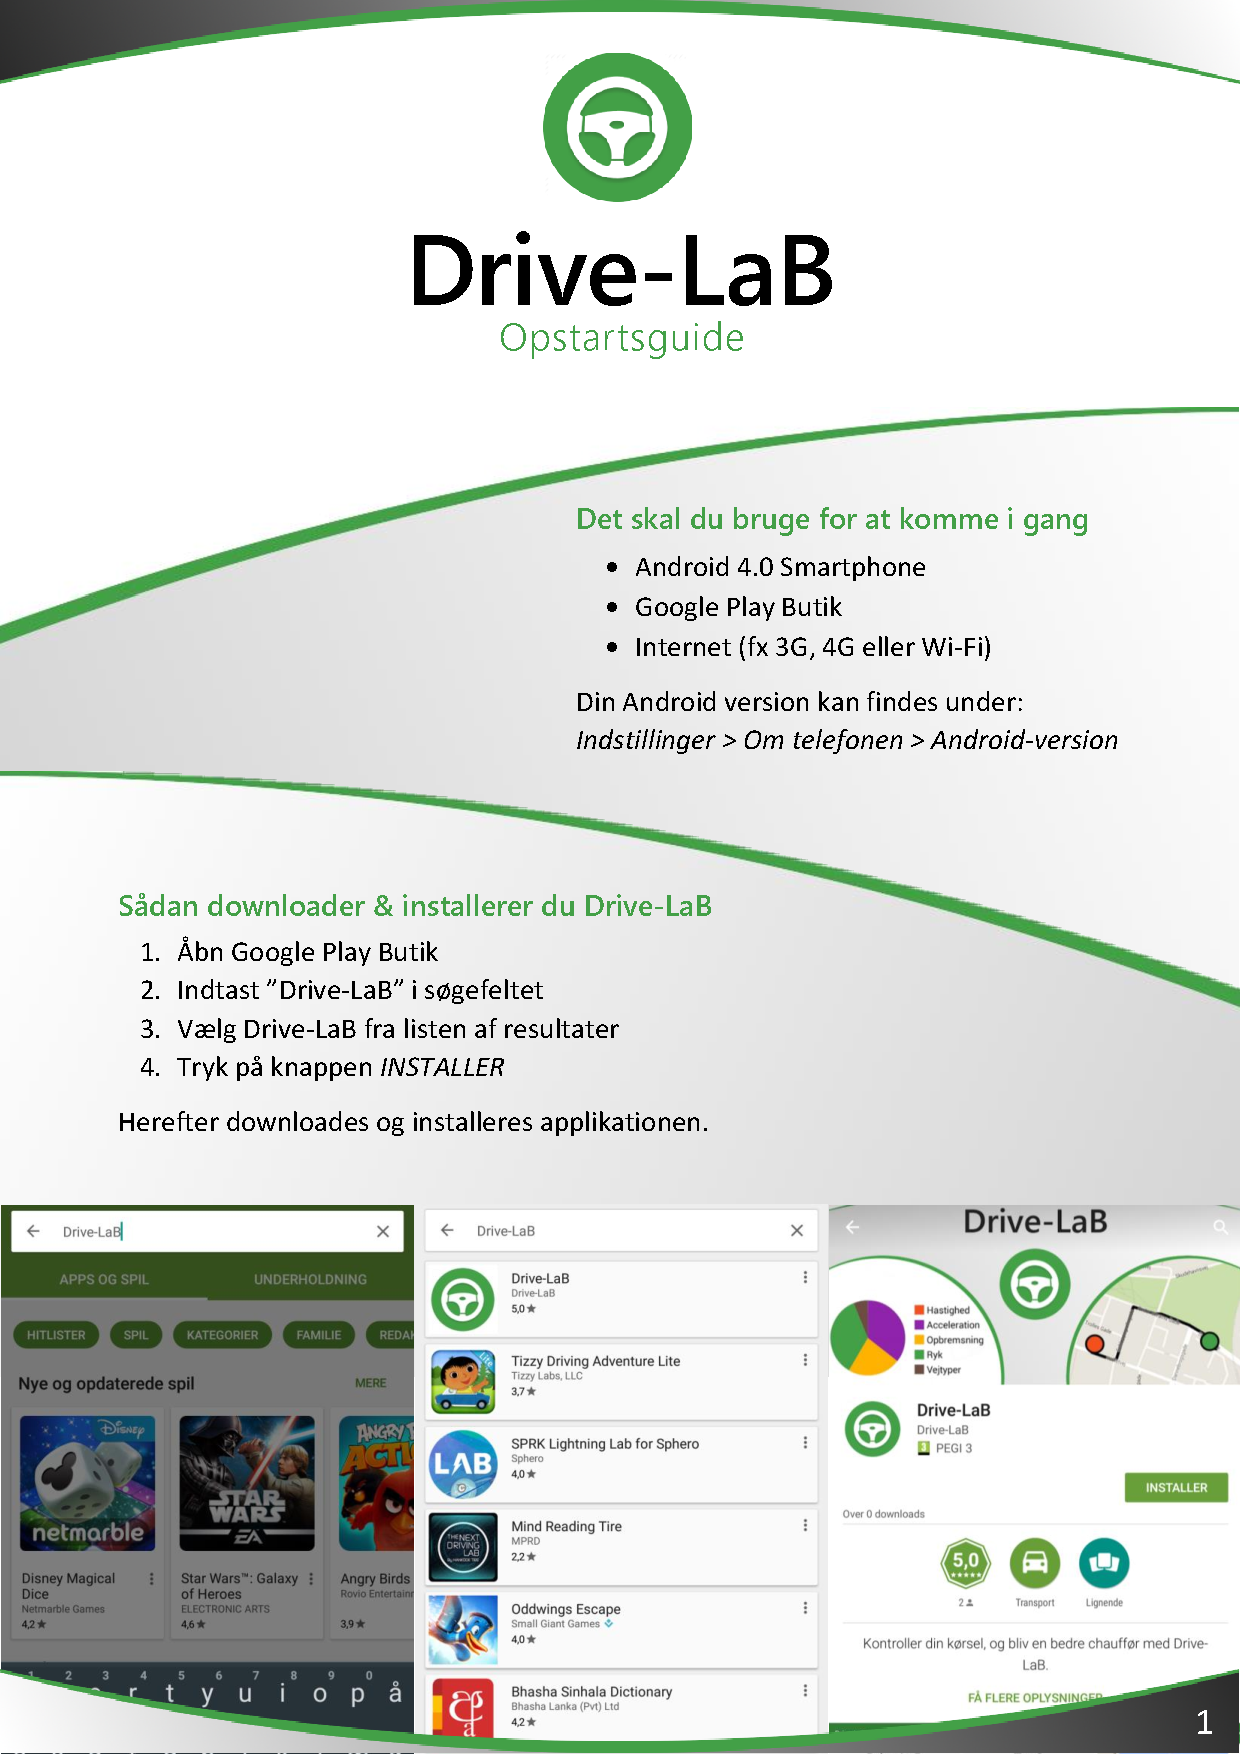
\includepdf[pages={1-}]{Appendix/Drive-LaB_Guide.pdf}
\subsection*{Data Warehouse}\label{app:datawarehouse}

\begin{figure}[tb]
\centering
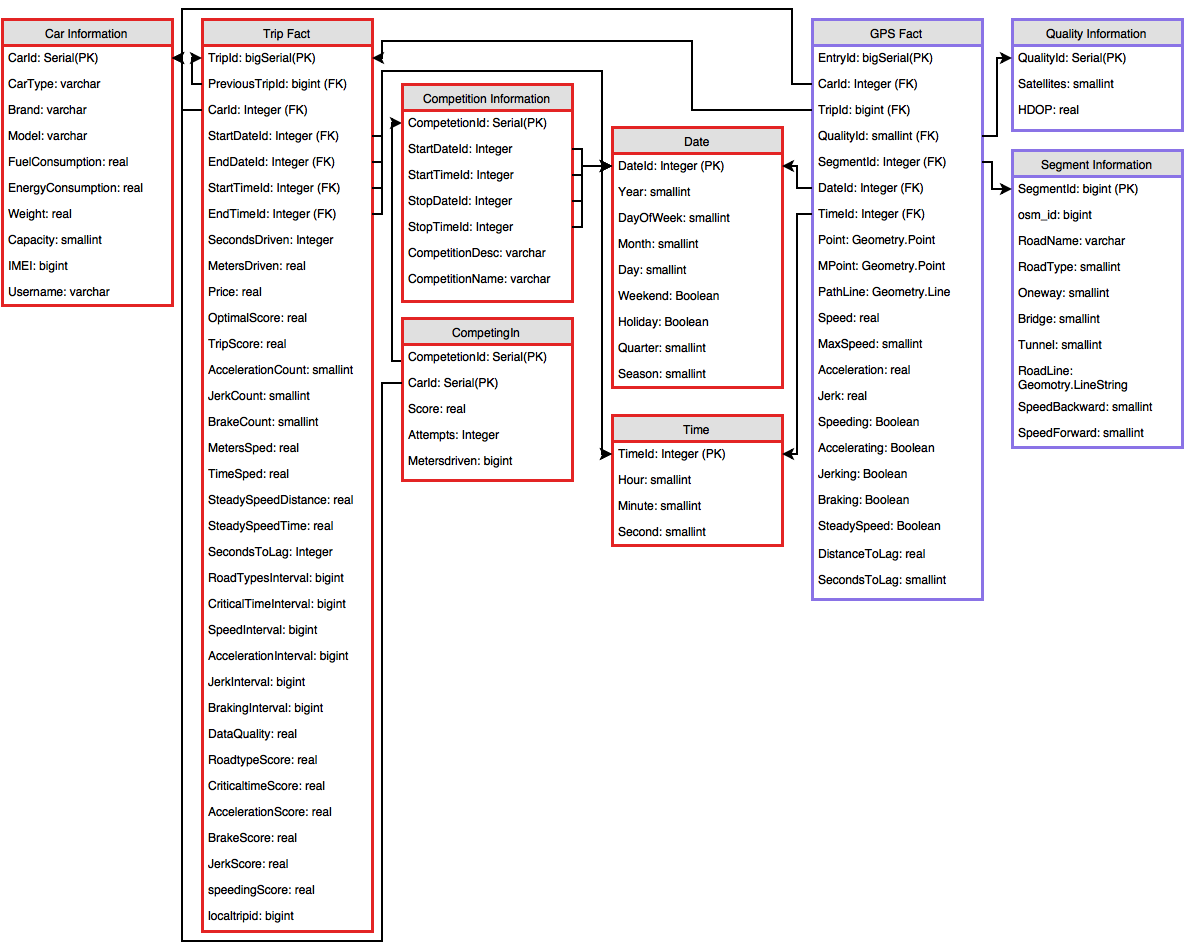
\includegraphics[width=0.95\textwidth]{Pictures/newdatawarehouse}
\caption{A picture of the entire data warehouse as it is used in the project}
\label{app:fig:newdatawarehouse}
\end{figure}

\end{document}